% !TEX root = ../../main_without_quantization.tex
\section{The Detailed Pipeline}
\label{chap:detailed_pipeline}

\subsection{Proposal Scoring}
\label{detailed:proposal}

\begin{figure}[H]
\centering
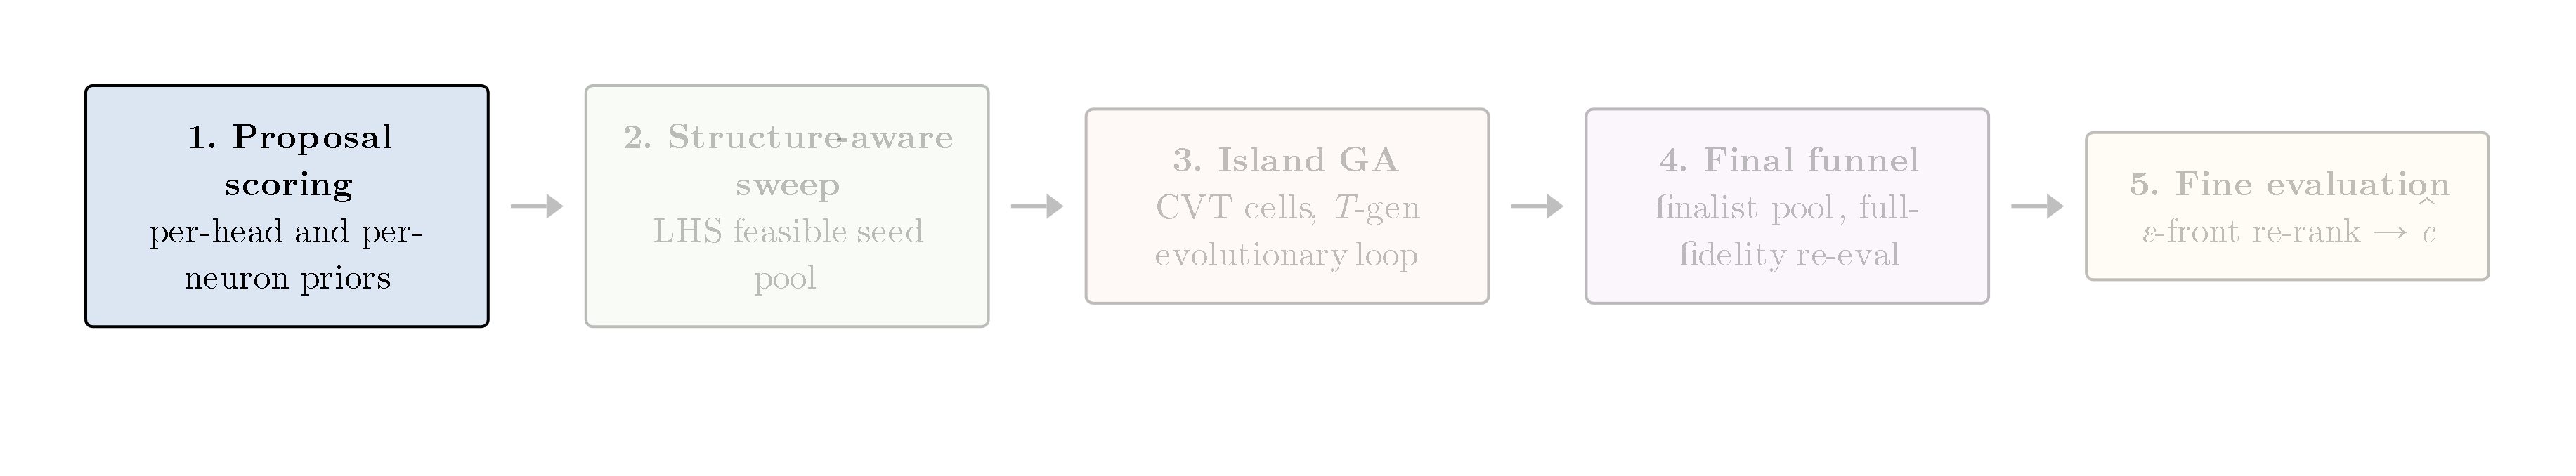
\includegraphics[width=0.85\linewidth]{figures/phase_banner_1.png}
\end{figure}

The first phase computes proposal scores before any candidate mask is sampled. These local saliency estimates make later discrete edits less arbitrary. The intuition follows classical pruning saliency: a unit is valuable when a small change to its gate would strongly affect the objective, or when removing it directly increases reconstruction error \citep{lecun1989optimal,hassibi1993second,molchanov2017variational,michel2022not}. Here the saliency is computed for heads and feed-forward neurons against the teacher's per-layer residual update target on the fixed metric subset.

For head $h$ of layer $\ell$, let $g_{\ell,h}(x)$ denote the gradient of the teacher-forced per-layer update target with respect to a multiplicative gate placed at head $(\ell,h)$ for calibration example $x$. This gradient measures local sensitivity: if the squared gradient is large, changing the gate of that head is expected to disturb the layer update. The head proposal score combines this local sensitivity with an explicit zero-out reconstruction term:
\[
s_H[\ell, h] \;=\; \mathbb{E}_{x \sim \mathcal{D}_{\mathrm{cal}}}\!\left[\, g_{\ell,h}(x)^2 \,\right] + \lambda \cdot \mathrm{MSE}\!\left( \widetilde\Delta^{(\teacher,\, h{=}0)}_{\ell}, \Dlt{\ell} \right),
\]
where $\lambda$ is a fixed mixing coefficient. The MSE term measures how much the teacher's per-layer update changes when head $(\ell,h)$ is zeroed. The neuron score $s_N[\ell,n]$ is defined analogously by placing the gate on feed-forward neuron $(\ell,n)$. Both scores are row-normalised per layer, so they rank units within the same layer rather than comparing raw magnitudes across layers.

The search also needs a layer-level score because the sweep and the repair routine sometimes decide which layers should remain active before they decide which exact units to keep. The per-layer aggregate
\[
\mathrm{imp}(\ell) \;=\; \sum_{h} s_H[\ell, h] \;+\; \sum_{n} s_N[\ell, n]
\]
gives this single importance number per layer. Phase~2 uses it when choosing active layers, and repair uses it to define the protected core.

Neuron mutation and repair operate on blocks rather than individual neurons. To make block addition and removal efficient, each layer receives a cumulative block table. For layer $\ell$, let $\pi_\ell$ be the permutation that sorts $s_N[\ell,\cdot]$ in descending order. The cumulative score of the first $b$ neuron blocks is
\[
S_\ell[b] \;=\; \sum_{j = 1}^{b \cdot b_n} s_N[\ell,\, \pi_\ell(j)], \qquad b = 0, 1, \ldots, \lfloor \nffn / b_n \rfloor.
\]
The marginal gain of adding the next block to layer $\ell$ is $S_\ell[b{+}1] - S_\ell[b]$, and the marginal loss of removing the current last block is $S_\ell[b] - S_\ell[b{-}1]$. After the one-time descending sort, both queries are constant-time. This matters during mutation and repair because many candidate edits require quick decisions about where to add or remove neuron capacity.

\begin{figure}[H]
\centering
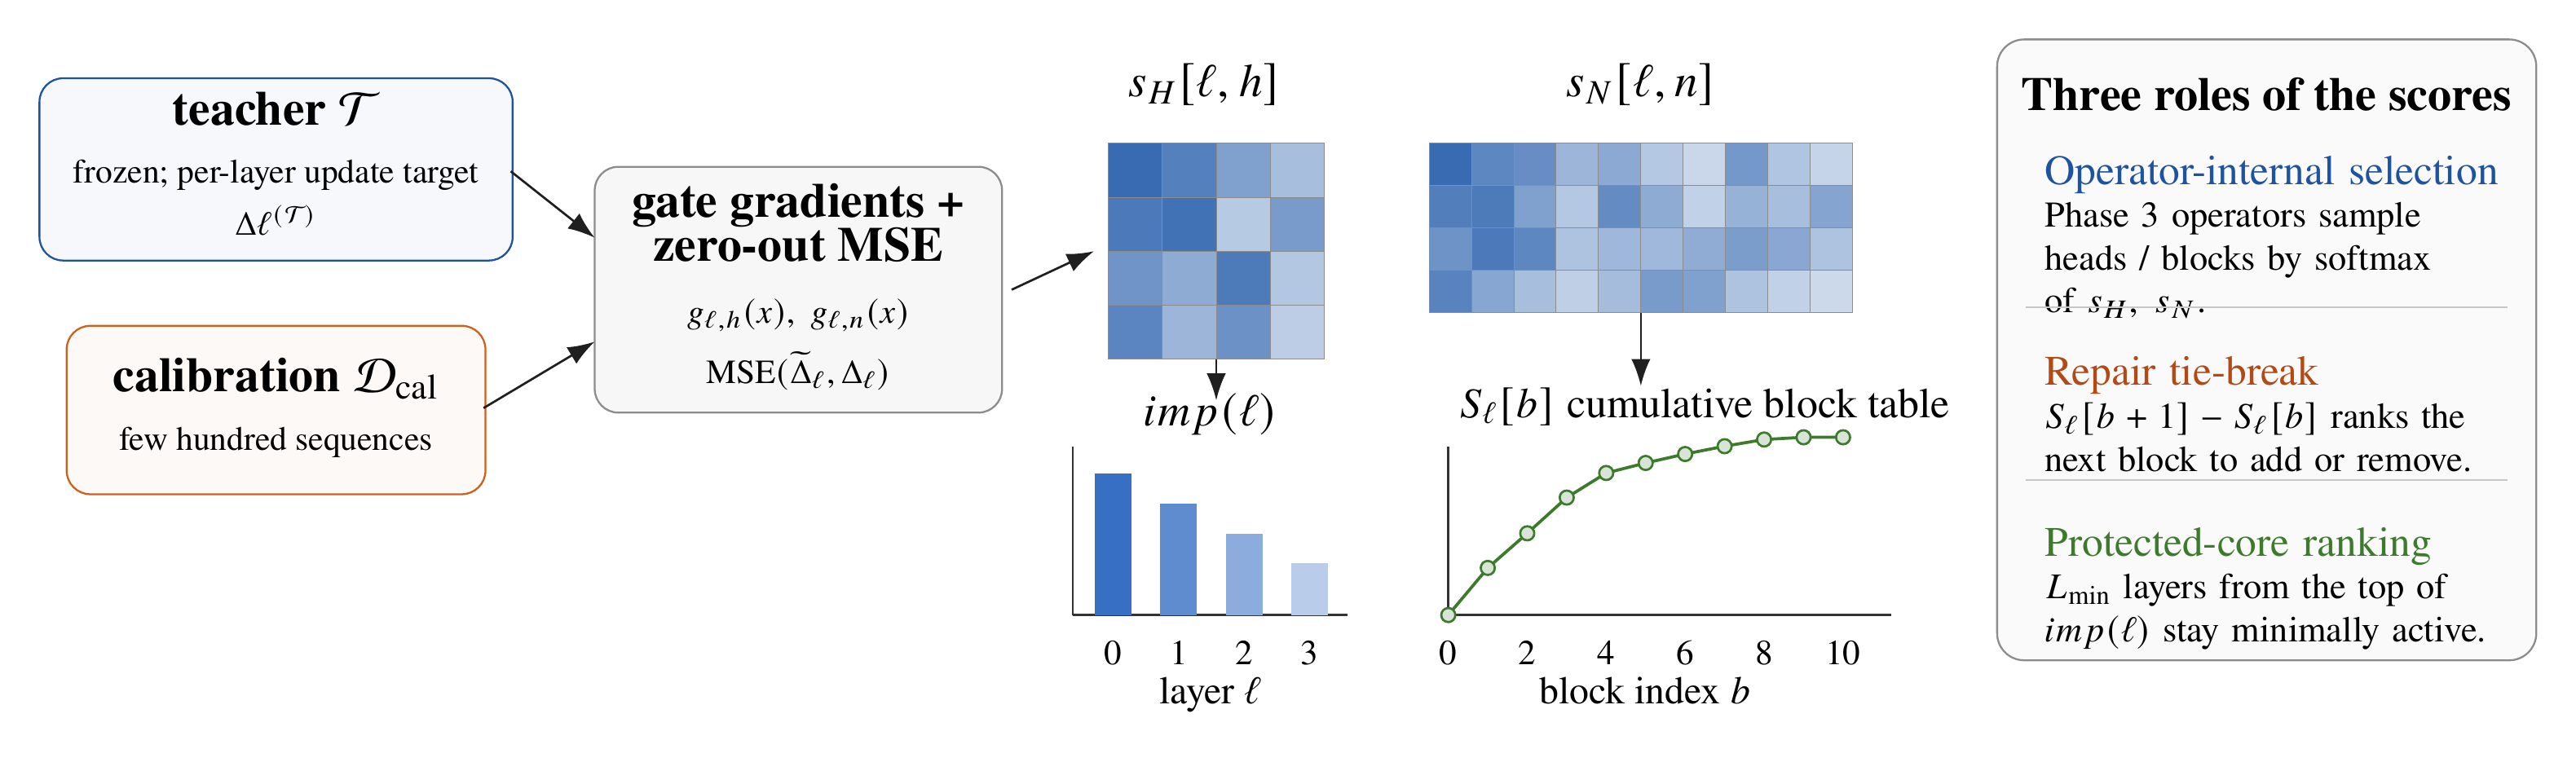
\includegraphics[width=0.95\linewidth]{figures/proposal_scoring.png}
\caption{Proposal scoring. For each calibration batch, gradients of the teacher's per-layer update target with respect to head and neuron gates yield squared sensitivities and a reconstruction MSE; their combination, row-normalised per layer, produces $s_H[\ell, h]$ and $s_N[\ell, n]$. Summing over each layer gives $\mathrm{imp}(\ell)$. Sorting $s_N[\ell, \cdot]$ in descending order and accumulating block sums yields the table $S_\ell[b]$, from which marginal gain and loss queries take $O(1)$.}
\label{fig:proposal_scoring}
\end{figure}

The scores then feed three parts of the search. The mutation operators of Phase~3 use $s_H$ and $s_N$ to define sampling probabilities when heads or neuron blocks are added, removed, or swapped. The repair routine uses $S_\ell$ to choose the best block to add or the least damaging block to remove when a candidate must be projected back into the feasible band. The guarded core during repair is formed from the $L_{\min}$ most important layers, so that repair cannot deactivate every high-priority layer while satisfying the budget.
\subsection{Initialisation: Structure-Aware Sweep}
\label{detailed:sweep}

\begin{figure}[H]
\centering
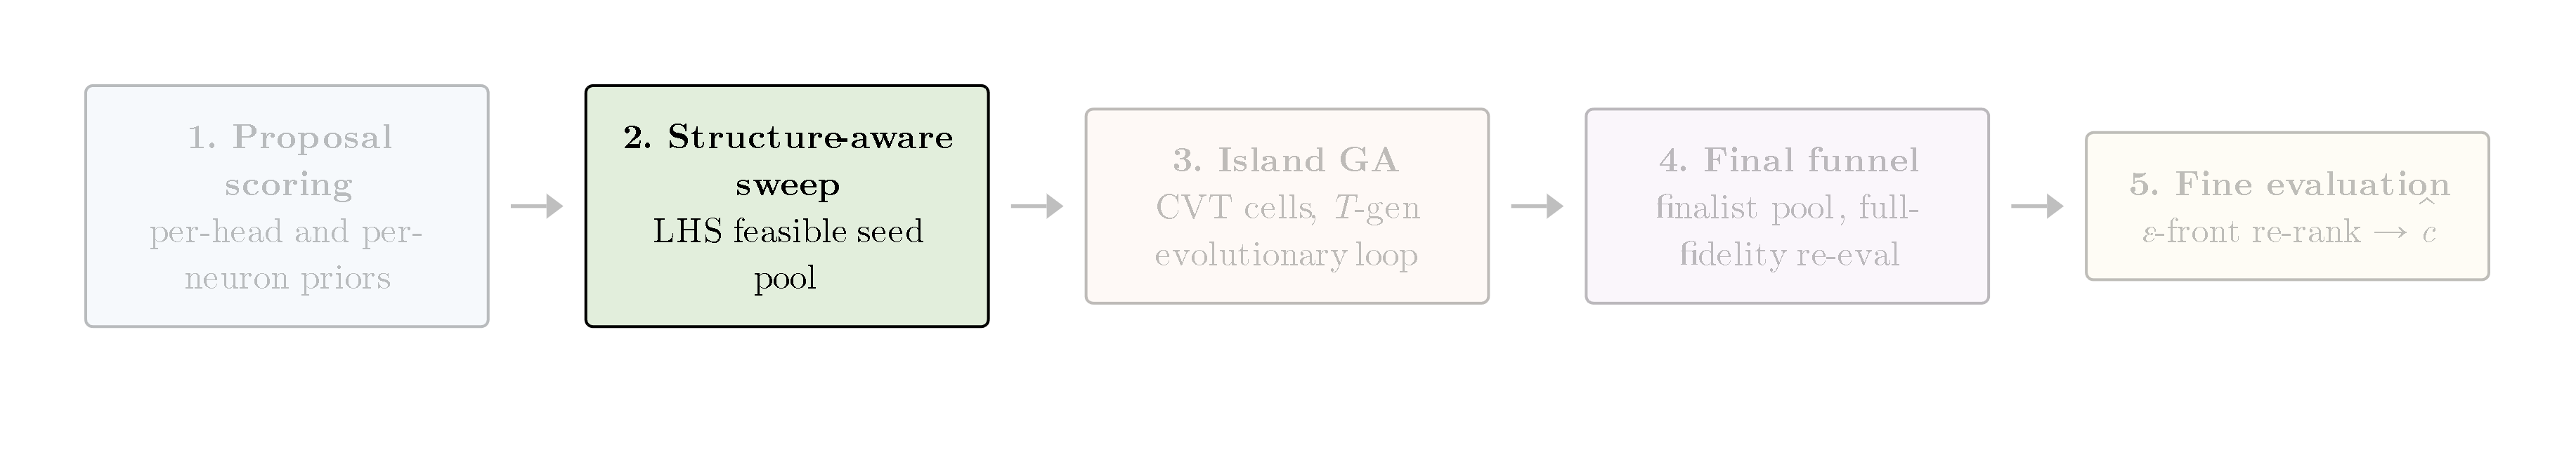
\includegraphics[width=0.85\linewidth]{figures/phase_banner_2.png}
\end{figure}

Proposal scores say which units look locally promising, but they do not yet give a diverse set of feasible architectures to search from. Phase~2 builds that set: a pool of masks inside $\mathcal{X}_\budget$ spread across qualitatively different allocations, since the island partition of Section~\ref{detailed:cvt} is fitted and seeded from it. Coverage comes from a stratified Latin hypercube design \citep{mckay1979comparison} over three macro axes, with each sampled point turned into one candidate.

The axes are the active-layer count $\nactive \in \{L_{\min}, \ldots, L_{\max}\}$, the head-MAC fraction $\phi_H$ that splits a layer's budget between attention and feed forward, and a subset mode that picks which $\nactive$ layers stay active from the importance vector $\mathrm{imp}(\ell)$, ranging from strictly top-scoring to uniformly random with an optional single-branch variant. The depth bound is the most minimally complete layers the budget allows,
\[
L_{\max}
=
\min\left(
\nlayers,
\left\lfloor
\frac{\budget}{\headcost + b_n\neuroncost}
\right\rfloor
\right),
\]
where $\headcost + b_n\neuroncost$ is the cost of one layer carrying a single attention head and a single block of feed-forward neurons.

Each design point becomes a mask in one pass, as summarised in Figure~\ref{fig:sweep_lhs}. The subset mode fixes the active set $A$; the budget is divided across $A$ in proportion to importance-weighted shares $\tilde w_\ell$, with a random perturbation on each weight so that repeated samples under the same prior still differ; and $\phi_H$ converts each layer's share into an integer head count and a block-aligned neuron count,
\[
\actl =
\mathrm{round}\!\left(
\frac{\phi_H \budget \tilde w_\ell}{\headcost}
\right),
\qquad
\nactl =
b_n
\left\lfloor
\frac{(1-\phi_H)\budget \tilde w_\ell}{b_n\neuroncost}
\right\rfloor .
\]
The retained head identities are sampled from $s_H[\ell,\cdot]$, and layers outside $A$ stay empty. Rounding can push the cost just outside the band, so a budget-repair step adds or removes block-aligned structures by proposal score until the candidate lies in $\mathcal{X}_\budget$. Repeating this over all samples gives the feasible seed pool used by the partition fit of the next phase \citep{du1999centroidal}.

The Latin hypercube is used only on the encoder, whose genome exposes a few interpretable meta-axes that can be stratified directly. The decoder genomes instead carry one axis per layer (Section~\ref{sec:other_candidate_forms}), around ninety discrete dimensions for the bit and rank vectors, where stratified sampling would need exponentially many full forward passes. Those searches stratify in the six-dimensional descriptor space through the CVT partition of Section~\ref{detailed:cvt}, which is cheap and adapts to where feasible genomes actually fall.

\begin{figure}[htbp]
\centering
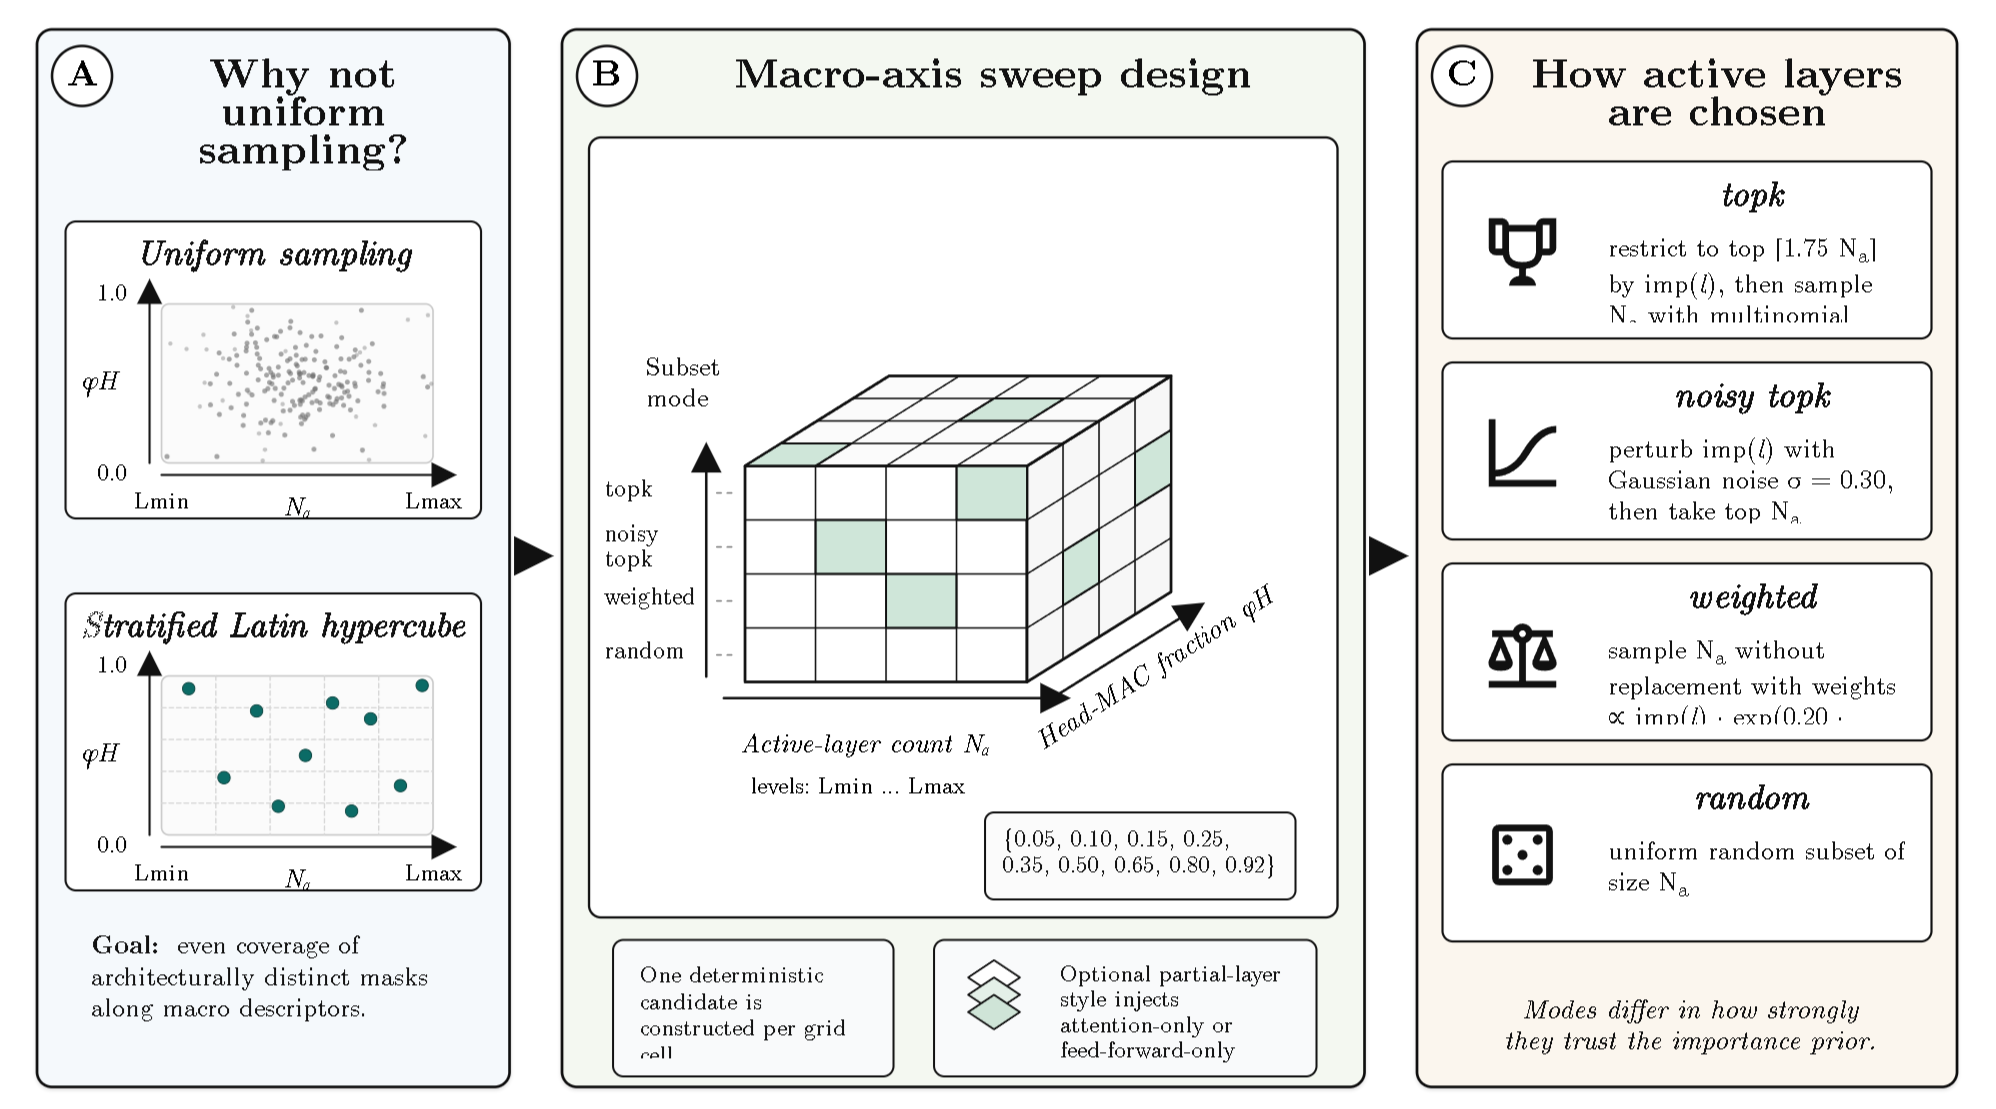
\includegraphics[width=0.95\linewidth]{figures/sweep_lhs.png}
\caption{Structure-aware sweep. Each sampled design point $(\nactive, \phi_H, \mathrm{mode})$ yields one candidate. The subset mode chooses the active layers from the layer importance scores; the head--neuron split $\phi_H$ divides the budget; and the importance-weighted per-layer allocation distributes the split into integer head counts and block-aligned neuron counts.}
\label{fig:sweep_lhs}
\end{figure}


\subsection{CVT Partition and Island Construction}
\label{detailed:cvt}

\begin{figure}[H]
\centering
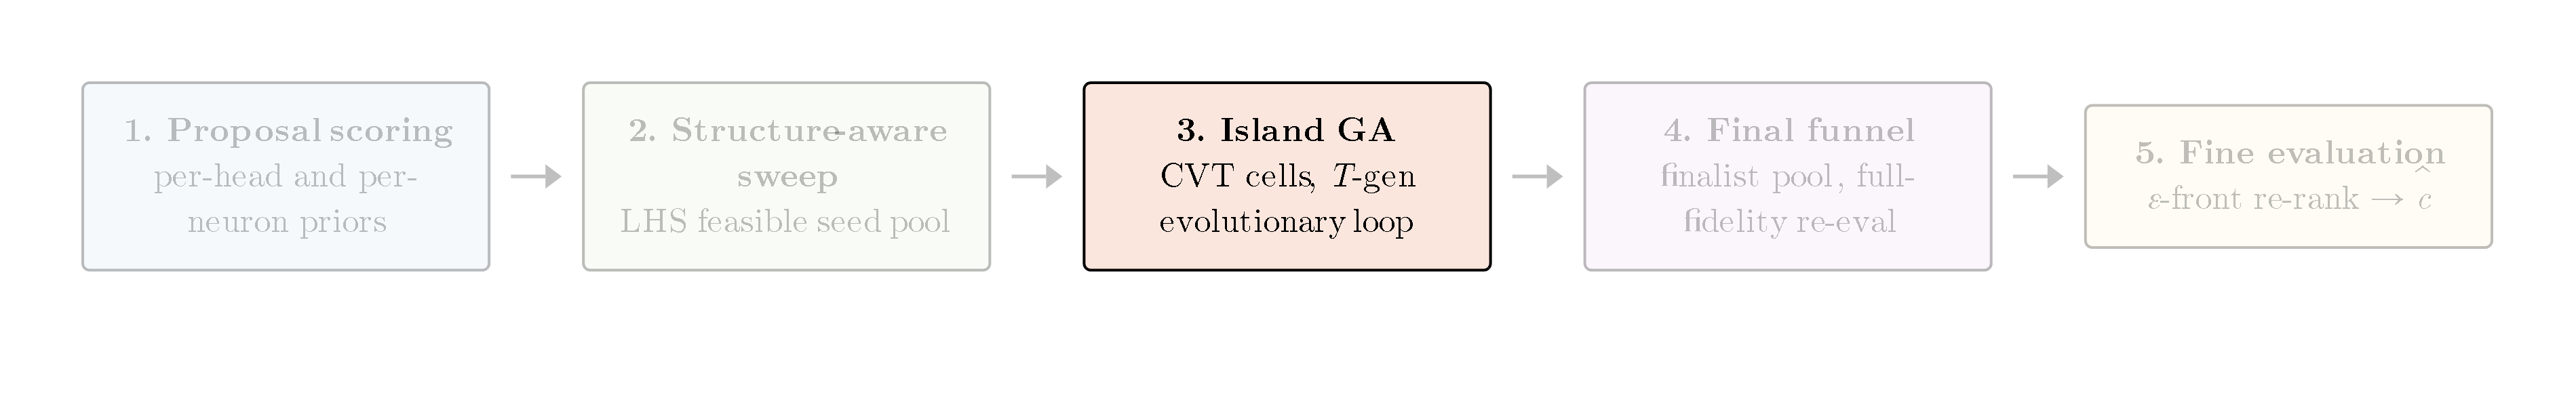
\includegraphics[width=0.85\linewidth]{figures/phase_banner_3.png}
\end{figure}

The sweep defined in Section~\ref{detailed:sweep} results in a scored feasible pool $\mathcal{S}=\{x_i\}_{i=1}^{M}$, where each $x_i$ lies within the budget band and has a surrogate distance $\Phi(x_i)$ from the teacher (Section~\ref{chap:metric}), with lower values being better. Sorting by quality alone is not sufficient to start the local search, because the top candidates can belong to different allocation regimes: some spend more budget on attention, some keep more feed-forward width, and some concentrate the budget into fewer active layers. A head swap or neuron transfer affects these regimes differently, so one mixed population can push edits that benefit one regime while harming another. Phase~3 therefore separates candidates by architecture and gives each region its own local population, or island \citep{cantupaz2000efficient}. Each island carries its own best solution so far and its own record of which edits have been working.

\paragraph{Architectural Descriptor.}
To group candidates by shape, each candidate is mapped to a six-dimensional descriptor vector, $z(x)=(z_1(x),\ldots,z_6(x))\in[0,1]^6$. For encoder pruning, Table~\ref{tab:cvt_descriptor} lists what each coordinate measures: how the budget splits between attention and feed forward, how many layers keep both branches active, how evenly the budget is spread across depth, and how high or low in the stack the attention and feed-forward capacity sits. For decoder searches, the same role is played by family-specific descriptors built from the layer-drop, bit-width, low-rank, or recovery level vectors. The closed-form expressions for the encoder and decoder descriptors are given in Appendix~\ref{sec:appendix_descriptors}.

This descriptor projects each possible candidate to a point in the six-dimensional shape space described above. That point is not yet a search region. It only says where the candidate sits relative to other candidates in terms of allocation, active depth, budget spread, and depth placement of capacity. The next step is therefore to cluster the descriptor cloud into a small set of regions whose members are structurally close. 

\begin{table}[H]
\centering
\footnotesize
\setlength{\tabcolsep}{4pt}
\begin{tabularx}{0.92\textwidth}{c l X}
\toprule
Coordinate & Quantity & Interpretation \\
\midrule
$z_1$ & attention MAC share & separates head-heavy from neuron-heavy allocations \\
$z_2$ & surviving feed-forward width & measures how much dense feed-forward capacity remains \\
$z_3$ & complete active-layer fraction & measures how much depth retains both branches \\
$z_4$ & budget entropy across layers & distinguishes spread-out and concentrated allocations \\
$z_5$ & head centre of mass & locates attention capacity along depth \\
$z_6$ & neuron centre of mass & locates feed-forward capacity along depth \\
\bottomrule
\end{tabularx}
\caption{Six encoder descriptor coordinates used to partition the feasible sweep pool.}
\label{tab:cvt_descriptor}
\end{table}

\paragraph{Descriptor Standardisation and CVT Fitting.}
The descriptor now gives a common language for architecture shape. Before distance-based clustering is applied, the descriptor coordinates are standardised because their empirical spreads can differ across the sweep pool. For every candidate $x_i\in\mathcal{S}$,
\[
\tilde z_i=\frac{z(x_i)-\bar z}{\sigma_z+\epsilon},
\]
where $z(x_i)$ is the descriptor of sweep candidate $x_i$, $\bar z$ is the componentwise sample mean, $\sigma_z$ is the componentwise sample standard deviation, $\epsilon$ avoids division by zero, and $\tilde z_i$ is the standardised descriptor used for clustering. Standardisation places all six coordinates on a common numerical scale.

The standardised descriptors are then partitioned by a \emph{Centroidal Voronoi Tessellation} (CVT) \citep[Appendix~\ref{sec:appendix_cvt}]{du1999centroidal}. The fitting procedure uses farthest-point seeding followed by Lloyd iterations, as in $k$-means clustering \citep{lloyd1982least,macqueen1967classification}. The first centre $\tilde\mu_1$ is drawn uniformly from the standardised seed descriptors $\{\tilde z_i\}$. Each following centre is chosen from the part of the descriptor cloud farthest from the centres already selected:
\[
\tilde\mu_{j+1}
:=
\arg\max_{\tilde z_i}
\min_{1\le q\le j}
\|\tilde z_i-\tilde\mu_q\|_2^2 .
\]
This farthest-point construction places each new centre in the part of descriptor space least covered by the centres already selected. Lloyd's assignment step then maps each descriptor to its closest centre,
\[
\mathrm{label}(i)
:=
\arg\min_{1\le j\le K}
\|\tilde z_i-\tilde\mu_j\|_2^2,
\]
and the update step replaces each centre by the mean descriptor assigned to it:
\[
\tilde\mu_j
\leftarrow
\frac{1}{|C_j|}
\sum_{i\in C_j}\tilde z_i,
\qquad
C_j=\{i:\mathrm{label}(i)=j\}.
\]
Assignment and update are repeated until the labels stop changing. The final centres are mapped back to the original descriptor coordinates by
\[
\mu_j=(\sigma_z+\epsilon)\tilde\mu_j+\bar z .
\]
The resulting cells are nearest-centre regions in descriptor space:
\[
V_j
:=
\left\{
z\in[0,1]^6:
\|z-\mu_j\|_2
\le
\|z-\mu_q\|_2
\text{ for all }q\ne j
\right\}.
\]
Each cell groups candidates with similar allocation shape. These cells provide the regions from which island populations are constructed.

% \paragraph{Basins.}
% The cells are useful as geometric regions, but the search edits masks directly. Each cell must therefore be converted into constraints that can be checked after an offspring is created. The candidates assigned to a cell also give it a plain name: a cell whose masks spend most of the budget on attention is \emph{head-heavy}, one that keeps most of the budget in feed-forward width is \emph{neuron-heavy}, one that keeps only a few layers active is \emph{layer-sparse}, and the rest are \emph{balanced}. These names are only for reference; the search itself uses numeric ranges. For cell $j$, those ranges form a basin $\mathcal{B}_j$: the smallest and largest head count and neuron count seen in the cell, the range of the attention-cost share, the range of per-layer cost, the smallest fraction of the budget a member must actually spend, and the cell centre $\mu_j$ together with a radius $r_j$ that sets how far a mask's descriptor may lie from $\mu_j$ and still count as belonging to the cell. After an operator edits a mask, a projection step pulls the edited mask back inside these ranges and re-applies the budget repair of Section~\ref{detailed:sweep}, so the offspring keeps both the shape of its cell and a feasible budget. Keeping the basins separate is what stops every island from drifting into the same allocation pattern.

\paragraph{Island Seeding.}
With the CVT cells fixed, each cell receives its own island population. The candidates assigned to cell $j$ are sorted by the surrogate distance $\Phi$ defined in Section~\ref{chap:metric}, where lower values are better. The strongest feasible candidates are copied into that island. If a cell contains too few candidates, additional candidates are taken from nearby cells to complete the initial population. Each island then carries the running state
\[
\mathcal{I}_j=(\pop_j,\; x_j^\star,\; d_j^\star,\; \mathcal{A}_j),
\]
namely its population $\pop_j$ of $P$ feasible masks, the best mask $x_j^\star$ found in the cell so far with its distance $d_j^\star$, and a selector $\mathcal{A}_j$ that learns which edit operator to try next in this cell from how much each operator improved candidates in the past \citep{auer2002nonstochastic,neu2015explore}. Phase~3 therefore begins with one population per cell, each one starting from a different way of spending the same budget (Figure~\ref{fig:cvt_partition}).

\begin{figure}[H]
\centering
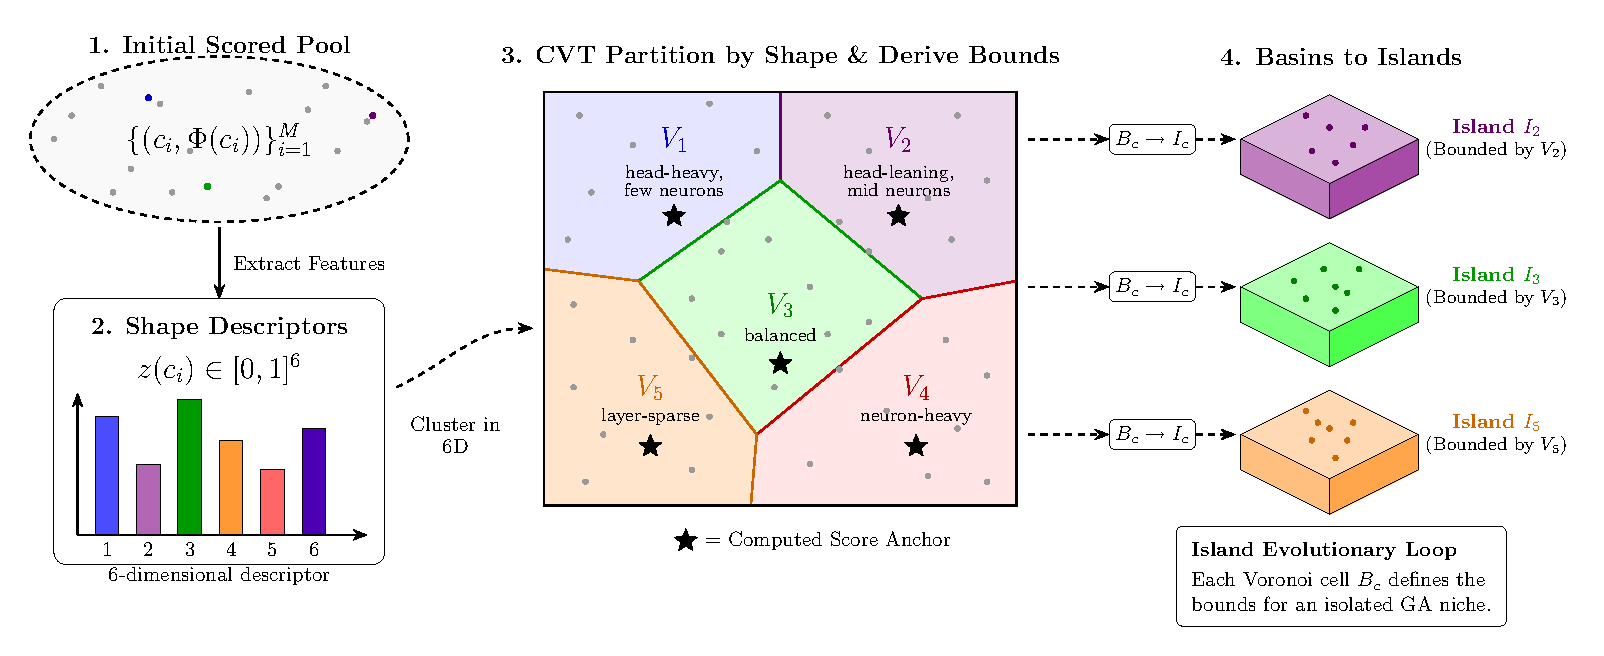
\includegraphics[width=0.95\linewidth]{figures/sweep_to_island.pdf}
\caption{From scored sweep candidates to islands. Sweep candidates are projected into the $(z_1, z_3)$ plane on the left and form a continuous cloud. The centre-based clustering step assigns each descriptor to its nearest centre and updates each centre to the mean of its assigned descriptors. This produces Voronoi cells. Each cell becomes a basin $\mathcal{B}_j$ on the right; the best scored candidates assigned to that basin seed the island $\mathcal{I}_j$, and the island then evolves with its own population, best-so-far candidate, and operator-selection bandit.}
\label{fig:cvt_partition}
\end{figure}


\subsection{Operator Library}
\label{detailed:operators}
\begin{figure}[H]
	\centering
	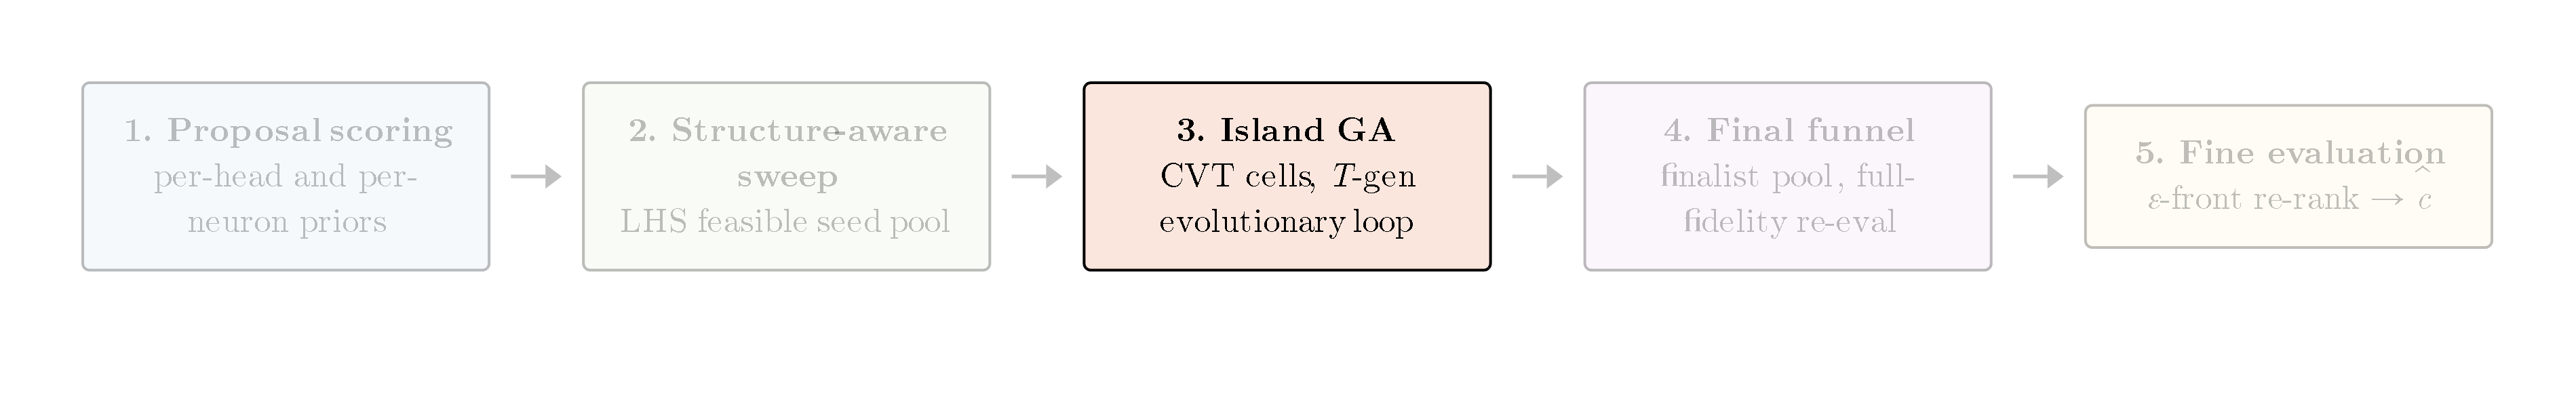
\includegraphics[width=0.85\linewidth]{figures/phase_banner_3.png}
\end{figure}

Now that we have the cells and populations set up, we need to explore the controlled variation on each island. The search utilizes two mutation scales. First is a local, small edit which refines a candidate within the current basin of attraction. Local edits will tend to preserve the global architecture, swapping units of similar cost. The second mutation size is structural, which changes the pattern of allocation (for example changing the active depth or the distribution of computation). This way an island can refine a local mask but also explore broader architectures as local refinement yields no new off-spring.

A Micro mutation is a local exchange of one unit for another, for example a budget-neutral head swap in the structural pruning of the encoder takes out one active head and adds in another head of the same cost, of course as mentioned before the proposal scores of the encoder model $s_H$ guides what head is added/ removed with higher chances for low importance units to be removed. Macro mutation involves a larger structural change, for example a layer-rewiring mutation switches between the set of active layers whilst remaining within the budget and active-depth constraint after projection.

The decoder searches reuse this two-scale design, with each task carrying its own family of operators. As one example from each, the layer-drop family can swap a dropped sub-block for a kept one, the quantization family can swap bit-width between two layers, and the low-rank family can swap rank between two layers. The full family for each task, encoder and decoder, is listed in Appendix~\ref{sec:appendix_operators}.

Crossover is another operators used. Mutation changes one of the parents into another; on the contrary, crossover takes two parents to produce one offspring. The function of crossover is to recombine beneficial layer assignments discovered in two different contexts. One parent can provide the active layer topology while the other may provide branch widths or layer wise count and the produced offspring is then mapped back to the basin, since it can be mapped to a valid looking mask whose cost or basin descriptor might be out of range.

When generating an offspring from existing parents, the algorithm either uses mutation or crossover, according to the operator mode. If it is mutation, then the bandit described in Section~\ref{detailed:bandit} is used to select an operator from the corresponding family. If it is crossover, then two parents are merged and the child is passed through the same feasibility projection used for generated offspring before evaluation. In this sense, the operator set contains the set of local or structural modifications; crossover provides recombination between already existing candidates.



\subsection{Bandit and Niche Conditioning}
\label{detailed:bandit}
\begin{figure}[H]
	\centering
	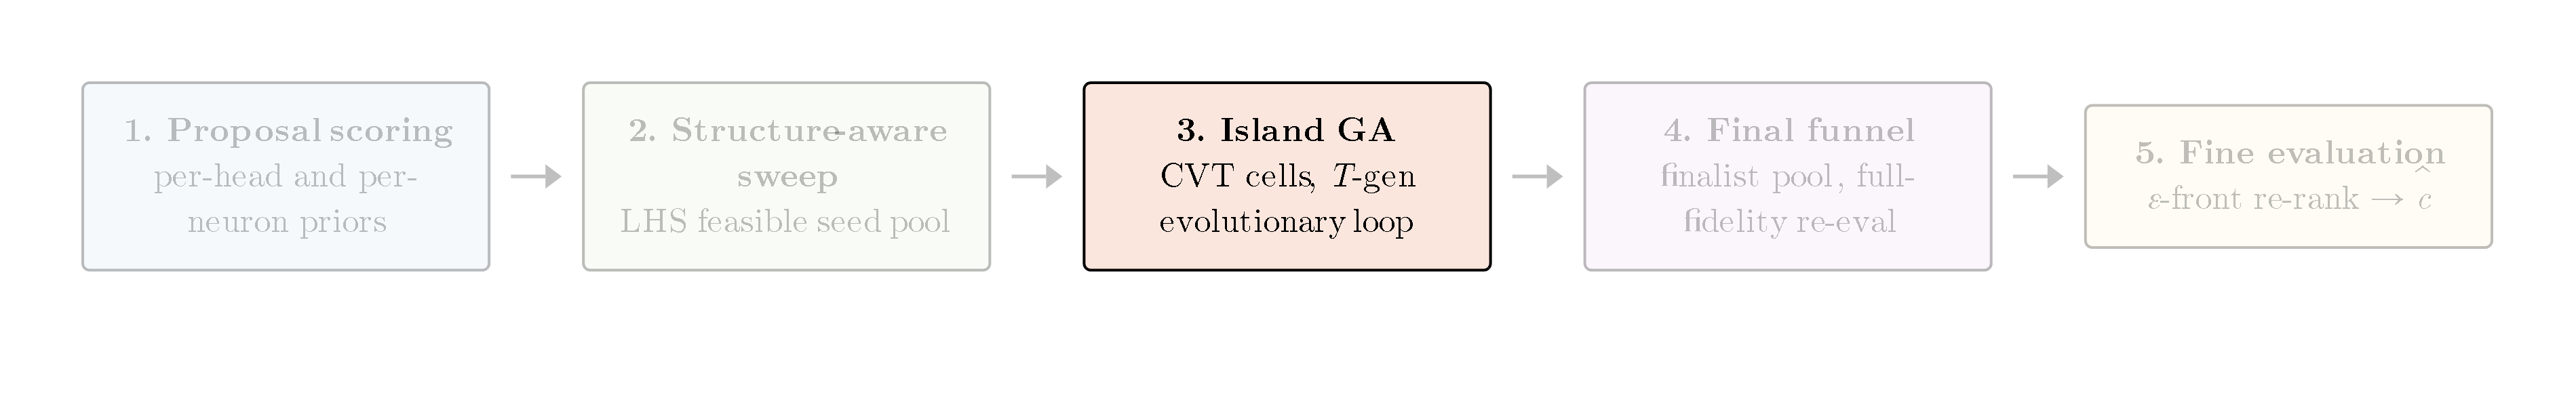
\includegraphics[width=0.85\linewidth]{figures/phase_banner_3.png}
\end{figure}

Once the operator families are defined, each island must decide which move to apply when producing offspring. This is treated as an operator-selection problem, with one EXP3-IX bandit per island \citep[see Appendix~\ref{sec:appendix_exp3ix}]{auer2002nonstochastic,neu2015explore}. For island $i$, the bandit stores a positive weight $w_i[o]$ for each operator $o$, and these weights define the base sampling distribution
\[
p_i[o]
=
(1-\gamma)
\frac{w_i[o]}{\sum_{o'}w_i[o']}
+
\frac{\gamma}{K},
\]
where $K$ is the number of available operators and $\gamma$ is the exploration coefficient. The learned term favours operators with larger accumulated weight; the uniform term keeps every operator selectable. After an offspring is evaluated, only the sampled operator receives reward, so the update uses the implicit-exploration estimate
\[
\hat r_o
=
\frac{r_o}{\hat p+\gamma}.
\]
Here, $\hat p$ is the probability used to sample operator $o$. The island then applies the multiplicative update
\[
w_i[o]
\leftarrow
w_i[o]\,
\exp\!\left(
\frac{\gamma\hat r_o}{K}
\right).
\]
This is the EXP3-IX update. The extra $\gamma$ in the denominator limits the size of reward estimates for rarely sampled operators, and weights are periodically rescaled for numerical stability.

The initial weights encode the cell focus obtained in Section~\ref{detailed:cvt}: depth-changing, attention-shifting, feed-forward-shifting, and balanced operators can start with different priors depending on the cell centroid. These priors only initialise the search; the multiplicative updates can override them once the observed rewards disagree.

For encoder pruning, the island-level bandit is further conditioned by a coarse parent niche because the head--neuron mask space can collapse toward repeated active-depth and allocation patterns. The niche is $\nu(\cand)=(\nactive,\;\mathrm{mac\_bucket},\;\mathrm{shape\_bucket})$: active depth, relative-cost bucket $\macop(\cand)/\budget$, and head-versus-neuron utilisation bucket. For each pair $(\nu,o)$, the island maintains the exponentially weighted reward average $\mathrm{ema}_i[\nu,o]\leftarrow(1-\eta_{\mathrm{ema}})\mathrm{ema}_i[\nu,o]+\eta_{\mathrm{ema}}r_o$. When a parent has niche $\nu$, the base probability $p_i[o]$ is reweighted by this niche statistic and renormalised:
\[
\tilde p_i[o;\nu]
\propto
p_i[o]\,
\big(0.5+\mathrm{ema}_i[\nu,o]\big),
\qquad
\mathrm{ema}_i[\nu,o]\in[0,1].
\]
The resulting distribution $\tilde p_i[\cdot;\nu]$ combines island-level evidence with parent-specific evidence. The reward $r_o$ is assigned after the offspring is compared with its parent by the two-step cohort rule of Section~\ref{metric:cohort}; a small extra bonus is added when the offspring also improves the island's best-so-far candidate.


\subsection{The Generation Loop}
\label{detailed:generation_loop}
\begin{figure}[H]
	\centering
	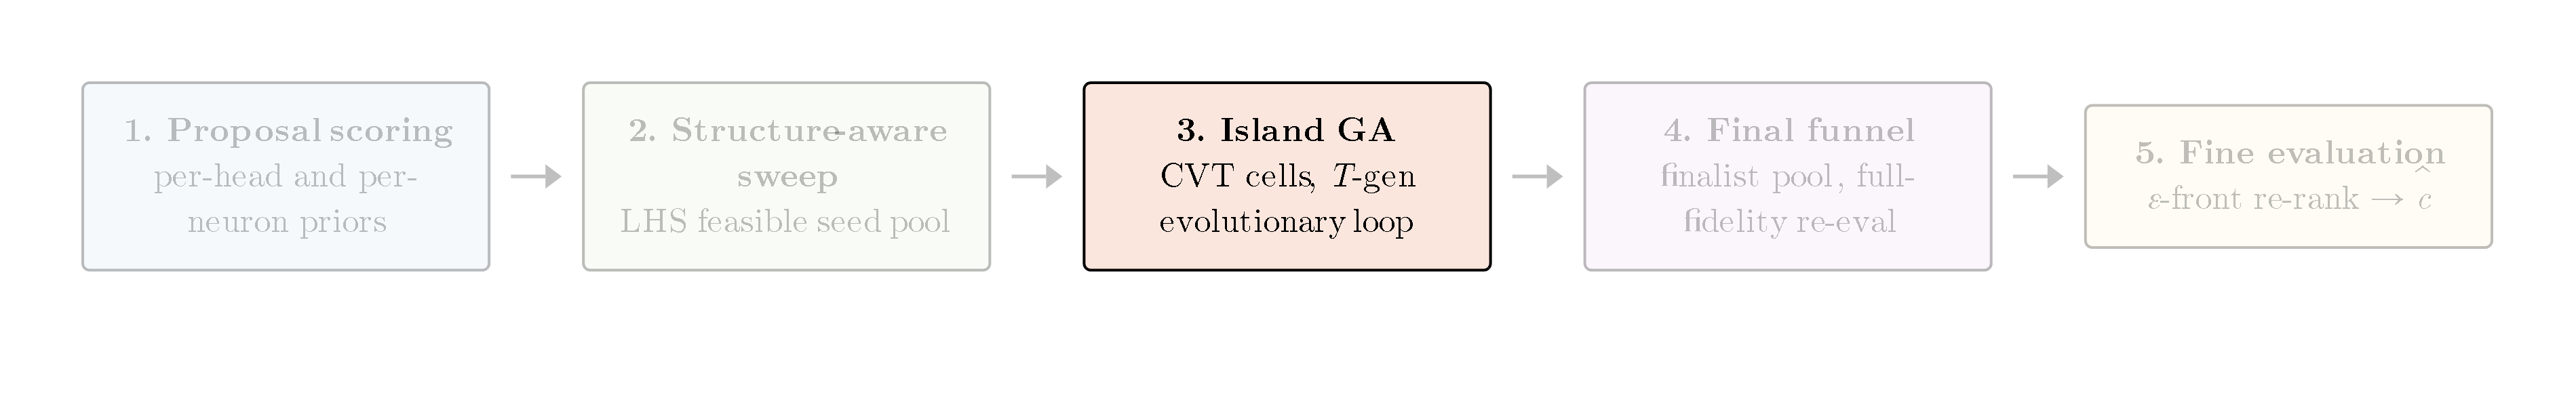
\includegraphics[width=0.85\linewidth]{figures/phase_banner_3.png}
\end{figure}

With the islands initialised and the operator distributions in place, the search enters the main generational loop of Phase~3. One generation updates every island once. The loop has a fixed order: score the current population, select parents, preserve elites, generate offspring, project them into the basin, evaluate them, apply the cohort rule, update the population, and pass strong candidates to the archives of Section~\ref{detailed:archives}.

\paragraph{Population Scoring.}
At the start of generation $t$, island $i$ holds a population
\[
\pop_i^{(t)} = \{\cand_{i,1}, \ldots, \cand_{i,P}\},
\]
all of whose members satisfy the basin constraints of Section~\ref{detailed:cvt}. The loop first evaluates every candidate at cheap fidelity on the calibration packs, producing a surrogate distance $\score(\cand_{i,j})$. Since lower distance is better, the distance is converted into a maximisation-oriented raw fitness
\[
f_{i,j} = -\,\score(\cand_{i,j}).
\]
This raw fitness ranks candidates by quality inside the current island. Before parent selection, it is corrected for crowding so that a dense group of near-identical masks does not dominate the parent pool.

The correction is a standard fitness-sharing rule. The distance $D_{jk}$ is the normalised Hamming distance between the exact binary mask signatures of candidates $\cand_{i,j}$ and $\cand_{i,k}$ in the same island, and $\sigma_s$ is the sharing radius. The shared fitness of candidate $j$ is
\[
\tilde f_{i,j}
\;=\;
\frac{f_{i,j}}{
1 + \sum_{k \ne j} \max\!\left(0, 1 - \frac{D_{jk}}{\sigma_s}\right)
}.
\]
Candidates surrounded by many near-duplicates receive lower selection strength. More isolated candidates retain more of their raw fitness. This keeps the island from collapsing too quickly onto one local shape.

\paragraph{Parent Selection and Elites.}
Parent selection is then applied on top of the shared fitness. The candidate pool is formed from the highest shared-fitness members of the island. Parents are drawn by repeated tournament selection. If the algorithm has already chosen parents $p_1,\ldots,p_{k-1}$ for the current offspring batch, then a tournament candidate $\cand_{i,j}$ receives the score
\[
S_{i,j}^{\mathrm{parent}}
\;=\;
\tilde f_{i,j}
\;+\;
\alpha_{\mathrm{nov}}
\min_{k' < k} D_{j,p_{k'}}
\;+\;
\alpha_{\mathrm{tie}}u,
\qquad
u \sim \mathrm{Unif}[0,1].
\]
The second term is a novelty bonus weighted by $\alpha_{\mathrm{nov}}$; among candidates with similar shared fitness, it favours candidates far from the parents already chosen for the same batch. The final term is a small random tie-break weighted by $\alpha_{\mathrm{tie}}$, used only to avoid deterministic cycles.

Before any offspring are created, the island preserves a small elite set unchanged. If the global elite budget is $\mathrm{elite\_size}$ and the number of islands is $I$, then island $i$ copies forward
\[
e = \left\lceil \frac{\mathrm{elite\_size}}{I} \right\rceil
\]
top candidates from $\pop_i^{(t)}$ directly into the next population. The remaining slots are filled with offspring. The fraction of those offspring allocated to macro operators is controlled by a schedule $\beta_M(t)$. Early generations emphasise broader structural edits. Later generations shift probability mass toward micro operators once each island has established its local region.

\paragraph{Offspring Generation and Evaluation.}
Each remaining population slot is filled independently. The bandit of Section~\ref{detailed:bandit} samples an operator with the niche-conditioned distribution $\tilde p_i[o;\nu]$ of the selected parent. A crossover-or-mutation decision then determines whether the child is produced from one parent by the sampled mutation operator or from two parents by crossover. In both cases, the child is projected back into the basin so that it satisfies the budget band and the island bounds.

For the decoder searches, this projection edits only the discrete level vector: dropped sub-block flags, bit-width levels, rank levels, or residual-rank allocations. The candidate is then materialised from the level database of Section~\ref{ga:level_db}, so evaluation loads precomputed weights or residual corrections rather than running quantization or SVD inside the search loop.

Before scoring, the offspring batch is filtered for repeated masks. Exact duplicates are removed by exact mask signature. A second pass removes structural near-duplicates using the same normalised mask distance and a deduplication radius $\sigma_d$. This prevents the offspring cohort from spending evaluations on masks that differ only by negligible local perturbations.

Every surviving offspring is evaluated at cheap fidelity. At scheduled generations, the strongest cheap-fidelity offspring are re-evaluated at full fidelity. If $\mathcal{D}_{\mathrm{cal}}^{\mathrm{full},r}$ denotes the $r$-th full calibration resample and $R$ the resample count, then the full-fidelity score used in the loop is
\[
\score^{\mathrm{full}}(\cand)
\;=\;
\frac{1}{R}\sum_{r=1}^{R} \score\!\left(\cand;\mathcal{D}_{\mathrm{cal}}^{\mathrm{full},r}\right).
\]
The cheap score remains the working ranking signal inside the generation. The full-fidelity pass provides a scheduled correction for candidates that already look competitive under the cheaper estimate.

\paragraph{Cohort Replacement and Rewards.}
The island then forms a cohort from incumbents and offspring and applies the two-step cohort rule of Section~\ref{metric:cohort}. Let
\[
\mathcal{C}_i^{(t)}
\;=\;
\pop_i^{(t)} \cup \mathcal{O}_i^{(t)}
\]
denote this combined set. The gate first removes candidates whose structural metric is unacceptable, then ranks the survivors with the task-facing terms defined by the surrogate metric. The next population $\pop_i^{(t+1)}$ is filled from this gated ranking after elite preservation. The same ranked cohort also supplies candidates for the archives described in Section~\ref{detailed:archives}.

The same gated score also defines the reward signal returned to the bandit. If operator $o$ produced offspring $\cand$ from parent $\cand^{\mathrm{par}}$, then its base reward is
\[
r_o
\;=\;
\mathbf{1}\!\left[
\score^{\mathrm{gate}}(\cand)
<
\score^{\mathrm{gate}}(\cand^{\mathrm{par}})
\right].
\]
A small additive bonus is applied when the offspring also improves the island best $\cand_i^\star$. The operator-selection rule is therefore rewarded for producing children that survive the same gated ranking used for population replacement.

\begin{figure}[H]
\centering
\resizebox{0.5\linewidth}{!}{%
\begin{tikzpicture}[
  box/.style={draw, rounded corners=2pt, align=center, minimum width=2.6cm, minimum height=0.82cm, fill=gray!7},
  side/.style={draw, rounded corners=2pt, align=center, minimum width=2.2cm, minimum height=0.78cm, fill=white},
  arr/.style={-{Latex[length=2mm]}, thick}
]
\node[box] (parents) {cheap evaluation of\\current population};
\node[box, below=0.7cm of parents] (select) {fitness sharing\\+ tournament with novelty};
\node[box, below=0.7cm of select] (operator) {bandit-sampled\\operator / crossover};
\node[box, below=0.7cm of operator] (project) {projection back\\into basin};
\node[box, below=0.7cm of project] (eval) {cheap evaluation\\+ scheduled full pass};
\node[box, below=0.7cm of eval] (gate) {cohort gate on\\incumbents + offspring};
\node[box, below=0.7cm of gate] (next) {next population};
\node[side, right=2.6cm of gate] (archives) {archive update\\Section~\ref{detailed:archives}};
\draw[arr] (parents) -- (select);
\draw[arr] (select) -- (operator);
\draw[arr] (operator) -- (project);
\draw[arr] (project) -- (eval);
\draw[arr] (eval) -- (gate);
\draw[arr] (gate) -- (next);
\draw[arr] (gate.east) -- (archives.west);
\end{tikzpicture}
}
\caption{One generation of Phase~3 inside a single island. The current population is scored, parents are selected with crowding correction and novelty, offspring are produced and projected back into the basin, the combined cohort is ranked by the two-step cohort rule of Section~\ref{metric:cohort}, and the surviving candidates form the next population. Archive updates use the same ranked cohort and are detailed in Section~\ref{detailed:archives}.}
\label{fig:generation_loop}
\end{figure}


\subsection{Archives}
\label{detailed:archives}


The generation loop updates the current population, but the search also preserves strong candidates across generations in three global archives. These archives have different purposes: one stores exact elites, one stores the non-dominated cost--distance frontier, and one stores representatives spread over a coarse descriptor grid.
\begin{figure}[H]
	\centering
	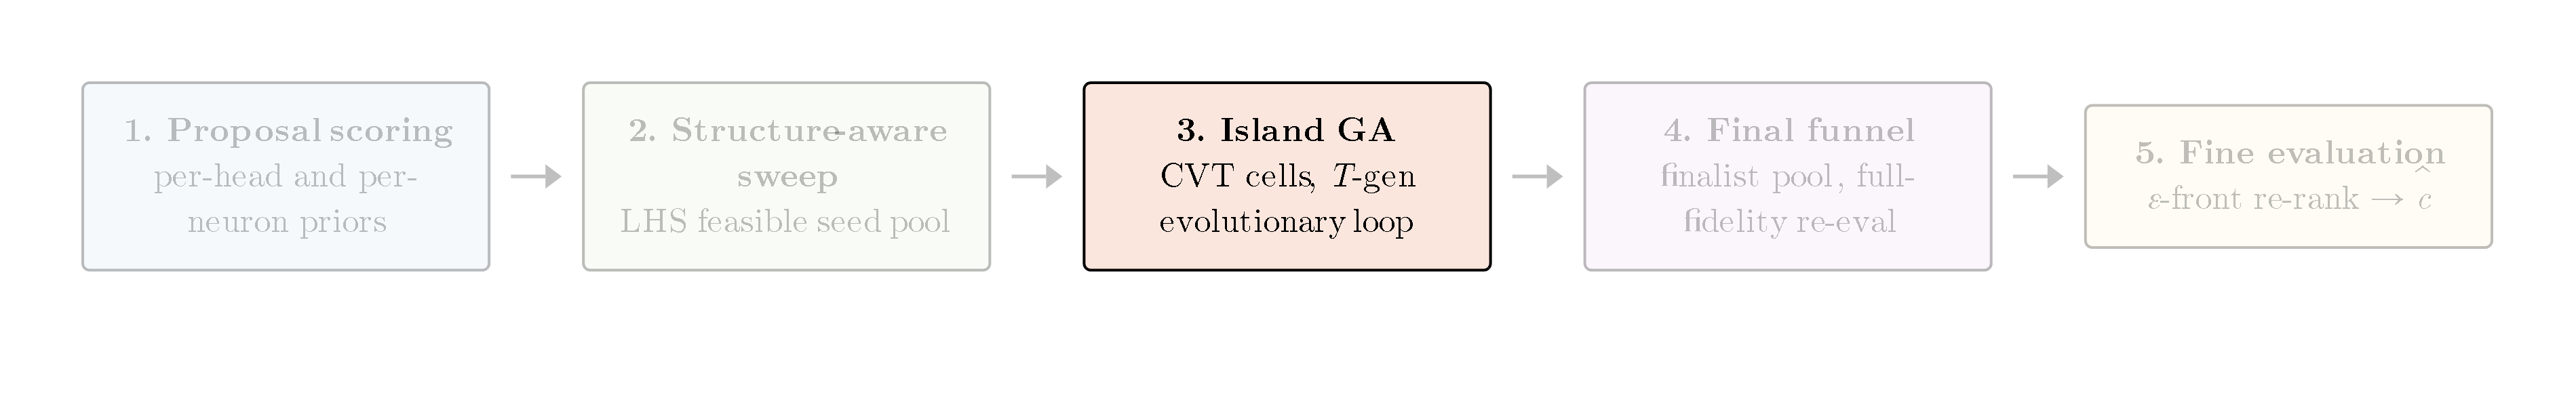
\includegraphics[width=0.85\linewidth]{figures/phase_banner_3.png}
\end{figure}
The Hall of Fame, denoted $\mathcal{H}$, is the strict elite memory. It has capacity $50$ and is deduplicated by exact mask signature. To prevent the archive from being monopolised by one macro pattern, it also enforces a per-signature cap of three entries for each macro signature. Here the macro signature is the pair formed by the active-layer set and the rounded head-MAC fraction,
\[
\operatorname{macro}(\cand)
\;=\;
\big(
\{\ell : \actl + \nactl > 0\},
\mathrm{round}(\phi_H(\cand), 0.1)
\big).
\]
Candidates enter $\mathcal{H}$ only if they improve on existing members under the gated search score and pass the exact-signature deduplication.

The Pareto archive, denoted $\mathcal{P}$, tracks the non-dominated frontier on the pair $(\score,\macop)$. A candidate $\cand_a$ dominates $\cand_b$ if
\[
\score(\cand_a) \le \score(\cand_b), \qquad \macop(\cand_a) \le \macop(\cand_b),
\]
and at least one of these inequalities is strict. The archive stores only non-dominated candidates and is capped at size $100$. This archive preserves alternatives that are not globally best in distance but remain competitive at a different point inside the budget band.

The MAP-Elites archive, denoted $\mathcal{M}$, stores one best-distance candidate per cell of a coarse grid on
\[
(\nactive,\; \mathrm{round}(\phi_H, 0.1)).
\]
If a candidate lands in a grid cell already occupied by another candidate, only the lower-distance one is kept. This archive preserves coverage across coarse depth and head-allocation patterns even when those patterns are not currently winning inside the islands.


\subsection{Final Funnel}
\label{detailed:final_funnel}
\begin{figure}[H]
	\centering
	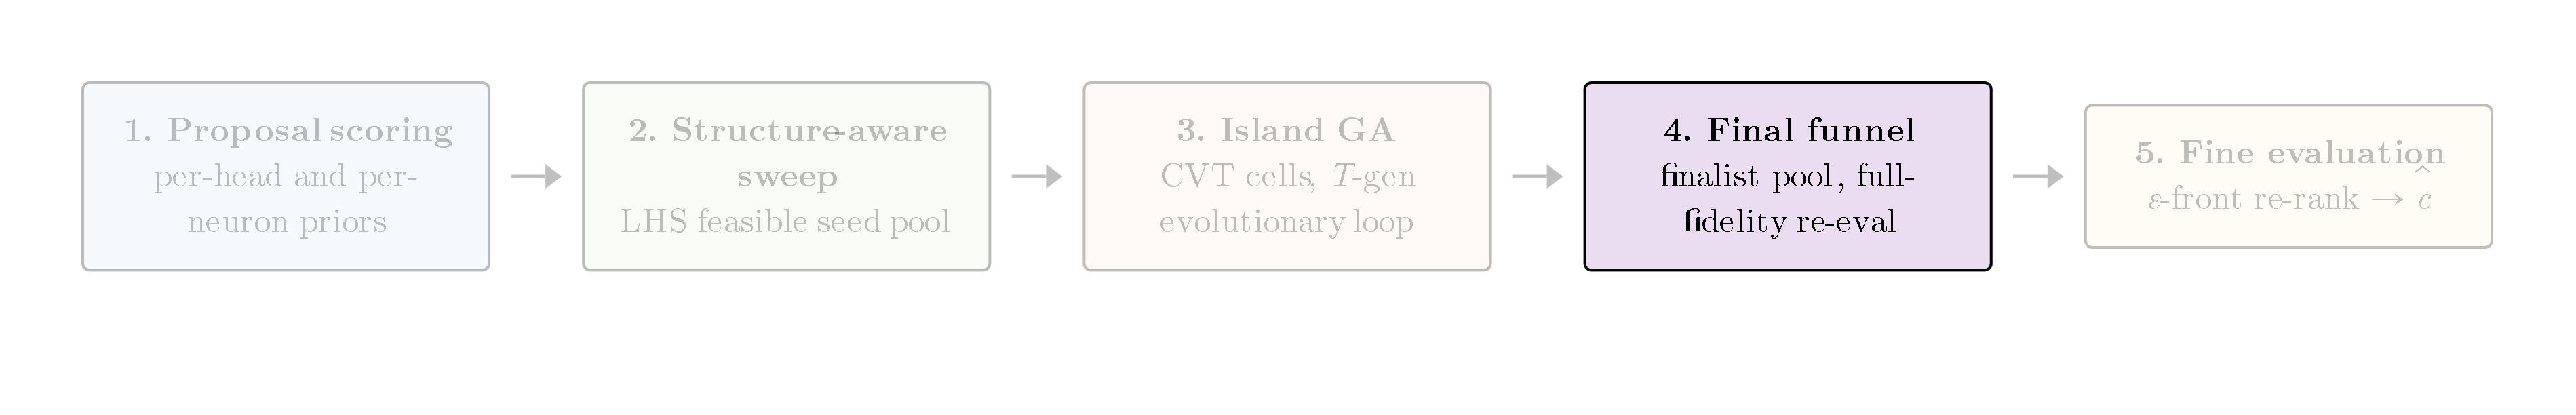
\includegraphics[width=0.85\linewidth]{figures/phase_banner_4.png}
\end{figure}

Once the generation loop finishes, the search no longer needs to maintain island populations. The remaining task is to gather the strongest candidates produced by the run into one finalist set and re-evaluate them at higher fidelity.

The finalist pool is assembled from the final incumbent, the top candidates of each island, and samples from the three archives. Writing $\widehat{\cand}^{(T)}$ for the best candidate observed by the end of generation $T$, the pool is
\[
\mathcal{F}
\;=\;
\{\widehat{\cand}^{(T)}\}
\cup
\bigcup_i \mathrm{top}_3(\pop_i)
\cup
\mathrm{sample}_5(\mathcal{H})
\cup
\mathrm{sample}_5(\mathcal{P})
\cup
\mathrm{sample}_5(\mathcal{M}).
\]
The union is then deduplicated by exact mask signature, so every finalist corresponds to a distinct binary architecture.

Each finalist is re-evaluated on the full calibration packs with $R_{\mathrm{final}} = 4$ independent resamples. The final score used in the funnel is
\[
\score^{\mathrm{final}}(\cand)
\;=\;
\frac{1}{R_{\mathrm{final}}}
\sum_{r=1}^{R_{\mathrm{final}}}
\score\!\left(\cand;\mathcal{D}^{\mathrm{full},r}_{\mathrm{cal}}\right).
\]
This final pass is more expensive than the generation-time evaluations, but it is applied only to the small finalist set that survives the funnel.


\subsection{Fine Evaluation and Selection}
\label{detailed:selection}
\begin{figure}[H]
	\centering
	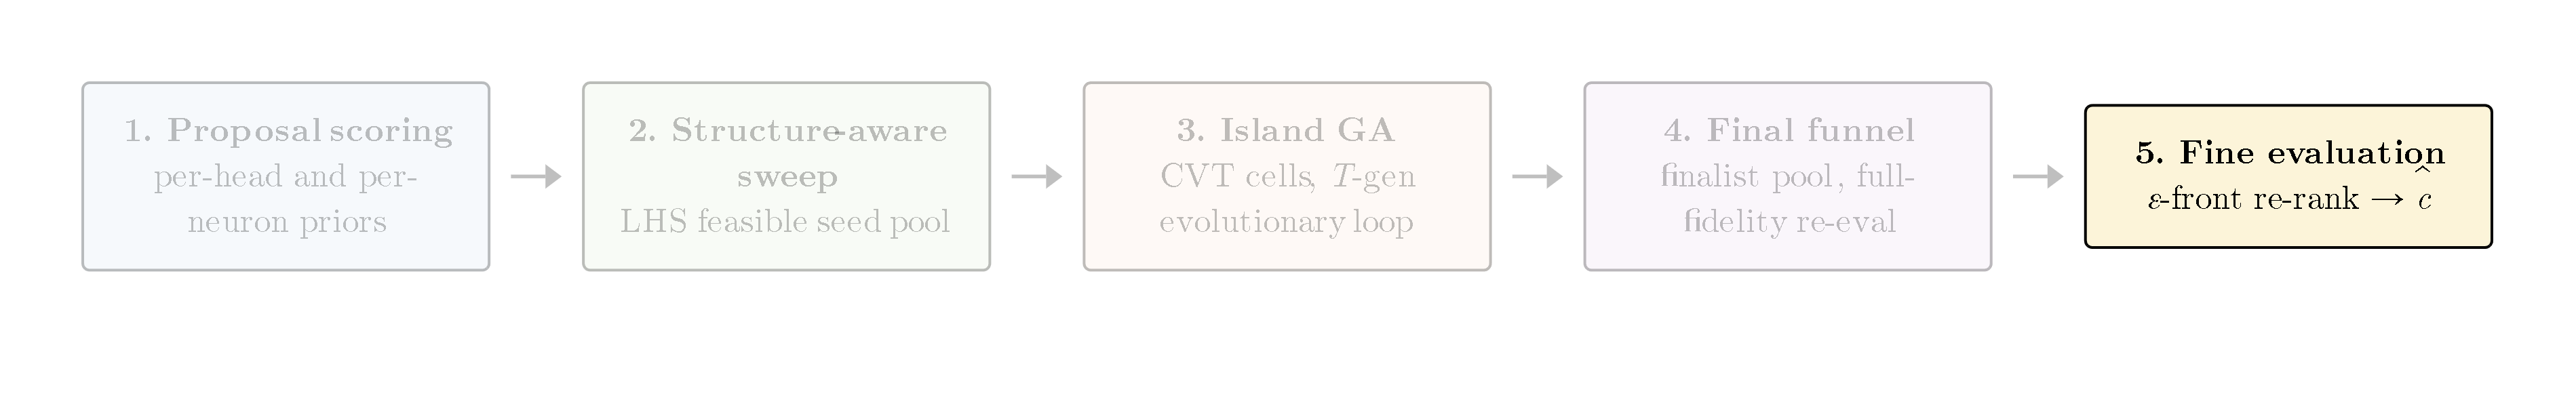
\includegraphics[width=0.85\linewidth]{figures/phase_banner_5.png}
\end{figure}

In the last pass, the distances are measured across many of the calibration tokens. Since the closest candidates can only be separated up to calibration noise, the winner is chosen among the $\epsilon$ front.

Let
\[
d^\star = \min_{\cand \in \mathcal{F}} \score^{\mathrm{final}}(\cand).
\]
The $\epsilon$-front is
\[
\mathcal{F}_\epsilon
\;=\;
\left\{
\cand \in \mathcal{F}
:
\score^{\mathrm{final}}(\cand) \le d^\star + \epsilon
\right\},
\qquad
\epsilon = 0.005.
\]
This keeps all finalists whose high-fidelity score is effectively tied with the best observed one.

The candidates in $\mathcal{F}_\epsilon$ are then sorted lexicographically by
\[
\big(\score^{\mathrm{final}}(\cand),\; -B_{\mathrm{use}}(\cand)\big).
\]
The first key prefers smaller final distance. The second key prefers the candidate that uses more of the allowed budget whenever two candidates are indistinguishable in final distance at the $\epsilon$ scale. Here $B_{\mathrm{use}}(\cand)$ denotes the used budget: MAC cost for encoder pruning, and the corresponding budget measure of the active decoder compression family. The selected architecture $\widehat{\cand}$ is the first element of this lexicographic order.

The procedure therefore ends with a single selected architecture $\widehat{\cand}$ obtained from the budget-constrained search. This completes the search stage itself. The selected architecture records the final compression decisions, but it does not by itself adapt the surviving parameters to that compressed form. When recovery is used, it is applied after search under the fixed architecture returned by the search.
